\documentclass[11pt]{article}
\usepackage[margin=1in]{geometry}
\usepackage{amsmath,amssymb,amsthm}
\usepackage{booktabs}
\usepackage{tikz}
\usepackage[hidelinks]{hyperref}

\newtheorem{theorem}{Theorem}
\newtheorem{lemma}[theorem]{Lemma}
\newtheorem*{sourceconj}{Conjecture 2 of Nie, Warmuth, Vishwanathan and Zhang}
\theoremstyle{remark}
\newtheorem{remark}{Remark}

\newcommand{\valD}{\operatorname{val}_D}
\newcommand{\val}{\operatorname{val}}
\newcommand{\Hh}{\hat H}

\title{The Sylvester--Hadamard game matrix does not have the largest boosting gap:\\
a counterexample to Conjecture~2 of Nie, Warmuth, Vishwanathan and Zhang}
\author{Qianghao Wu}
\date{27 November 2026}

\begin{document}
\maketitle

\begin{abstract}
Nie, Warmuth, Vishwanathan and Zhang (COLT 2013) view boosting as a zero-sum game and
build game matrices from Hadamard matrices. Let $\Hh$ be the $n\times n$ Hadamard matrix
with its first row removed. Their Conjecture~2 states that $\Hh$ gives the largest gaps
among all $(n-1)\times n$ matrices with entries $\pm1$ and game value~$0$: for every such
matrix $U$ and every $1\le t\le n$, the best $t$-column sub-matrix of $\Hh$ has a game value
at most that of the best $t$-column sub-matrix of $U$. We show that the conjecture is false
when $H$ is the Sylvester Hadamard matrix of order $n=16$. For $t=6$, the matrix $U$
obtained from the Hadamard matrix Had.16.3 of Sloane's library by deleting its all-ones
row satisfies $\max_{U_6}\valD(U_6)=-3/7$, while $\max_{\Hh_6}\valD(\Hh_6)\ge-1/3$. The
upper bound for $U$ comes from 8008 exact dual certificates, one for each set of 6
columns. Lean~4 with Mathlib checks the full statement from the definitions, with kernel
evaluation of the certificates and only the standard axioms. Two exact checkers in Python
also accept the certificates. The counterexample does not refute the weaker reading in which
$\Hh$ can come from any Hadamard matrix of order~$n$. This work has not yet been reviewed by
experts. The computations, the proofs and the text were produced by AI models (from
Anthropic and OpenAI), working under the author's direction.
\end{abstract}

\section{Introduction}

Boosting can be viewed as a zero-sum game between a row player and a column player
\cite{nie2013}. The rows of a game matrix are the examples, and the columns are the
hypotheses. After $t$ iterations, a boosting algorithm has seen $t$ columns, and the value of
the sub-matrix $U_t$ of these columns is the largest minimum margin that a convex
combination of them can reach. The source \cite{nie2013} asks how slowly this value can
approach the value of the full matrix. It defines the gap at step~$t$ as
$\val(U)-\max_{U_t}\val(U_t)$, where the maximum is over all sub-matrices of $t$ columns.
A large gap for every $t$ gives a lower bound for every boosting algorithm.

The source builds its game matrices from Hadamard matrices. For $n=2^k$ it takes the
$n\times n$ Hadamard matrix $H$, deletes the first row to get $\Hh$, and uses the game
matrix $\left[\begin{smallmatrix}\Hh\\-\Hh\end{smallmatrix}\right]$. It proves a lower bound
of $\sqrt{1/(2t)}$ on the gap for $1\le t\le n/2$ (its Theorem), and states two conjectures.
Conjecture~1 asserts a stronger lower bound of order $\sqrt{(\log n)/t}$ for
$\log n\le t\le cn$. Conjecture~2 asserts that $\Hh$ gives the largest gaps among all $\pm1$
matrices of value~$0$. The source reports that its authors verified Conjecture~2 ``by
tedious combinatorial arguments for $n=2,4,8$ and $t\le n$ as well as for $n=2^k$ and
$n-2\le t\le n$''.

\paragraph{Prior work.} Gr{\o}nlund, Larsen and Mathiasen \cite{gronlund2019} refuted
Conjecture~1. Their paper says ``Our main contribution is a refutal of this conjecture'', and
their algorithm SparsiBoost refutes the conjectured lower bound. Their paper does not
mention Conjecture~2. It is the only work in OpenAlex that cites \cite{nie2013}. We found
no claim of a settlement of Conjecture~2 in our searches (Section~\ref{sec:limits}).

\paragraph{Result.} Conjecture~2 is false for $n=16$ and $t=6$ when $H$ is the Sylvester
Hadamard matrix (Theorem~\ref{thm:main}). The counterexample $U$ is itself $\Hh'$ for a
different Hadamard matrix $H'$ of order~16. So the conjecture fails because the gap of the
Hadamard construction depends on the choice of the Hadamard matrix. The case
$(n,t)=(16,6)$ is outside the range that the source verified.

\section{Definitions and the conjecture}

We copy the definitions of the source \cite{nie2013}. For $t\ge1$ let
$S^t=\{w\in\mathbb{R}^t: w_j\ge0,\ \sum_j w_j=1\}$ be the probability simplex. For a matrix
$G$ with $t$ columns, equation~(1) of the source defines
\[
  \val(G)=\min_{d}\max_{w\in S^t} d^\top G w=\max_{w\in S^t}\min_r\,[Gw]_r .
\]
For a matrix $U$ the source writes $\valD(U)=\val\left(\left[\begin{smallmatrix}U\\-U
\end{smallmatrix}\right]\right)$ and notes that
\[
  \valD(U)=-\min_{w\in S^t}\|Uw\|_\infty\le 0 .
\]
Let $n=2^k$, let $H$ be the $n\times n$ Hadamard matrix, and let $\Hh$ be $H$ with its
first row removed. The conjecture is quoted word for word:

\begin{sourceconj}[{\cite[p.~3]{nie2013}}]
For any $(n-1)\times n$ dimensional $\pm1$ valued matrix $U$ satisfying $\valD(U)=0$, the
following inequality holds for $1\le t\le n$:
$\max_{\Hh_t}\valD(\Hh_t)\le\max_{U_t}\valD(U_t)$, where $\Hh_t$ is any $t$ column
sub-matrix of $\Hh$ and $U_t$ is any $t$ column sub-matrix of $U$.
\end{sourceconj}

\paragraph{The Hadamard matrix.} The source does not give a construction of ``the''
Hadamard matrix. For $n=2^k$ we use the Sylvester matrix
$H_{rc}=(-1)^{\langle r,c\rangle}$, $0\le r,c<n$, where $\langle r,c\rangle$ is the number
of common 1 bits of the binary forms of $r$ and $c$. Its first row is all $+1$, so $\Hh$
has row sums~0 and $\valD(\Hh)=0$, as the source's proof of its Theorem requires. This
reading is the one that we refute. Remark~\ref{rem:reading} discusses the other readings.

A ``$t$ column sub-matrix'' is the sub-matrix on $t$ distinct columns. Repeated columns
would not change the maximum for $U$: a repeated column adds nothing to the convex hull of
the columns.

\section{The counterexample}

Let $U$ be the $15\times16$ matrix in Figure~\ref{fig:matrices}. It is the Hadamard matrix
Had.16.3 of Sloane's library \cite{sloane} with its row~0 deleted. Row~0 of Had.16.3 is all
$+1$, so every row of $U$ has sum~0 and $[\mathbf 1^\top; U]$ is a Hadamard matrix. Written
with $+$ for $+1$ and $-$ for $-1$, the rows of $U$ (rows 1 to 15 of Had.16.3, read left to
right and then down) are
\begin{center}\small\ttfamily
\begin{tabular}{lll}
+-+-+-+-+-+-+-+- & ++--++--++--++-- & +--++--++--++--+\\
++++----++++---- & +-+--+-++-+--+-+ & ++----++++----++\\
+--+-++-+--+-++- & ++++++++-------- & +++-+------+-+++\\
++-+---+--+-+++- & ++---++---+++--+ & +-++-+---+--+-++\\
+-+---++-+-+++-- & +--++-+--++--+-+ & +---++-+-+++--+-
\end{tabular}
\end{center}

\begin{figure}[t]
\centering
% Generated by checks/draw.py. Do not edit.
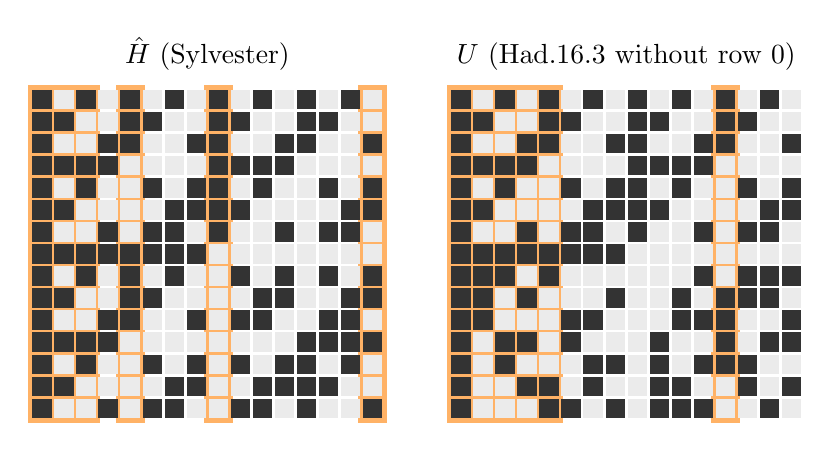
\begin{tikzpicture}[x=0.28cm,y=0.28cm]
\node[anchor=south] at (8,0.4) {$\hat H$ (Sylvester)};
\fill[orange!60] (-0.15,0.15) rectangle (1.15,-15.15);
\fill[orange!60] (0.85,0.15) rectangle (2.15,-15.15);
\fill[orange!60] (1.85,0.15) rectangle (3.15,-15.15);
\fill[orange!60] (3.85,0.15) rectangle (5.15,-15.15);
\fill[orange!60] (7.85,0.15) rectangle (9.15,-15.15);
\fill[orange!60] (14.85,0.15) rectangle (16.15,-15.15);
\fill[black!80] (0.06,-0.06) rectangle (0.94,-0.94);
\fill[black!8] (1.06,-0.06) rectangle (1.94,-0.94);
\fill[black!80] (2.06,-0.06) rectangle (2.94,-0.94);
\fill[black!8] (3.06,-0.06) rectangle (3.94,-0.94);
\fill[black!80] (4.06,-0.06) rectangle (4.9399999999999995,-0.94);
\fill[black!8] (5.06,-0.06) rectangle (5.9399999999999995,-0.94);
\fill[black!80] (6.06,-0.06) rectangle (6.9399999999999995,-0.94);
\fill[black!8] (7.06,-0.06) rectangle (7.9399999999999995,-0.94);
\fill[black!80] (8.06,-0.06) rectangle (8.94,-0.94);
\fill[black!8] (9.06,-0.06) rectangle (9.94,-0.94);
\fill[black!80] (10.06,-0.06) rectangle (10.94,-0.94);
\fill[black!8] (11.06,-0.06) rectangle (11.94,-0.94);
\fill[black!80] (12.06,-0.06) rectangle (12.94,-0.94);
\fill[black!8] (13.06,-0.06) rectangle (13.94,-0.94);
\fill[black!80] (14.06,-0.06) rectangle (14.94,-0.94);
\fill[black!8] (15.06,-0.06) rectangle (15.94,-0.94);
\fill[black!80] (0.06,-1.06) rectangle (0.94,-1.94);
\fill[black!80] (1.06,-1.06) rectangle (1.94,-1.94);
\fill[black!8] (2.06,-1.06) rectangle (2.94,-1.94);
\fill[black!8] (3.06,-1.06) rectangle (3.94,-1.94);
\fill[black!80] (4.06,-1.06) rectangle (4.9399999999999995,-1.94);
\fill[black!80] (5.06,-1.06) rectangle (5.9399999999999995,-1.94);
\fill[black!8] (6.06,-1.06) rectangle (6.9399999999999995,-1.94);
\fill[black!8] (7.06,-1.06) rectangle (7.9399999999999995,-1.94);
\fill[black!80] (8.06,-1.06) rectangle (8.94,-1.94);
\fill[black!80] (9.06,-1.06) rectangle (9.94,-1.94);
\fill[black!8] (10.06,-1.06) rectangle (10.94,-1.94);
\fill[black!8] (11.06,-1.06) rectangle (11.94,-1.94);
\fill[black!80] (12.06,-1.06) rectangle (12.94,-1.94);
\fill[black!80] (13.06,-1.06) rectangle (13.94,-1.94);
\fill[black!8] (14.06,-1.06) rectangle (14.94,-1.94);
\fill[black!8] (15.06,-1.06) rectangle (15.94,-1.94);
\fill[black!80] (0.06,-2.06) rectangle (0.94,-2.94);
\fill[black!8] (1.06,-2.06) rectangle (1.94,-2.94);
\fill[black!8] (2.06,-2.06) rectangle (2.94,-2.94);
\fill[black!80] (3.06,-2.06) rectangle (3.94,-2.94);
\fill[black!80] (4.06,-2.06) rectangle (4.9399999999999995,-2.94);
\fill[black!8] (5.06,-2.06) rectangle (5.9399999999999995,-2.94);
\fill[black!8] (6.06,-2.06) rectangle (6.9399999999999995,-2.94);
\fill[black!80] (7.06,-2.06) rectangle (7.9399999999999995,-2.94);
\fill[black!80] (8.06,-2.06) rectangle (8.94,-2.94);
\fill[black!8] (9.06,-2.06) rectangle (9.94,-2.94);
\fill[black!8] (10.06,-2.06) rectangle (10.94,-2.94);
\fill[black!80] (11.06,-2.06) rectangle (11.94,-2.94);
\fill[black!80] (12.06,-2.06) rectangle (12.94,-2.94);
\fill[black!8] (13.06,-2.06) rectangle (13.94,-2.94);
\fill[black!8] (14.06,-2.06) rectangle (14.94,-2.94);
\fill[black!80] (15.06,-2.06) rectangle (15.94,-2.94);
\fill[black!80] (0.06,-3.06) rectangle (0.94,-3.94);
\fill[black!80] (1.06,-3.06) rectangle (1.94,-3.94);
\fill[black!80] (2.06,-3.06) rectangle (2.94,-3.94);
\fill[black!80] (3.06,-3.06) rectangle (3.94,-3.94);
\fill[black!8] (4.06,-3.06) rectangle (4.9399999999999995,-3.94);
\fill[black!8] (5.06,-3.06) rectangle (5.9399999999999995,-3.94);
\fill[black!8] (6.06,-3.06) rectangle (6.9399999999999995,-3.94);
\fill[black!8] (7.06,-3.06) rectangle (7.9399999999999995,-3.94);
\fill[black!80] (8.06,-3.06) rectangle (8.94,-3.94);
\fill[black!80] (9.06,-3.06) rectangle (9.94,-3.94);
\fill[black!80] (10.06,-3.06) rectangle (10.94,-3.94);
\fill[black!80] (11.06,-3.06) rectangle (11.94,-3.94);
\fill[black!8] (12.06,-3.06) rectangle (12.94,-3.94);
\fill[black!8] (13.06,-3.06) rectangle (13.94,-3.94);
\fill[black!8] (14.06,-3.06) rectangle (14.94,-3.94);
\fill[black!8] (15.06,-3.06) rectangle (15.94,-3.94);
\fill[black!80] (0.06,-4.06) rectangle (0.94,-4.9399999999999995);
\fill[black!8] (1.06,-4.06) rectangle (1.94,-4.9399999999999995);
\fill[black!80] (2.06,-4.06) rectangle (2.94,-4.9399999999999995);
\fill[black!8] (3.06,-4.06) rectangle (3.94,-4.9399999999999995);
\fill[black!8] (4.06,-4.06) rectangle (4.9399999999999995,-4.9399999999999995);
\fill[black!80] (5.06,-4.06) rectangle (5.9399999999999995,-4.9399999999999995);
\fill[black!8] (6.06,-4.06) rectangle (6.9399999999999995,-4.9399999999999995);
\fill[black!80] (7.06,-4.06) rectangle (7.9399999999999995,-4.9399999999999995);
\fill[black!80] (8.06,-4.06) rectangle (8.94,-4.9399999999999995);
\fill[black!8] (9.06,-4.06) rectangle (9.94,-4.9399999999999995);
\fill[black!80] (10.06,-4.06) rectangle (10.94,-4.9399999999999995);
\fill[black!8] (11.06,-4.06) rectangle (11.94,-4.9399999999999995);
\fill[black!8] (12.06,-4.06) rectangle (12.94,-4.9399999999999995);
\fill[black!80] (13.06,-4.06) rectangle (13.94,-4.9399999999999995);
\fill[black!8] (14.06,-4.06) rectangle (14.94,-4.9399999999999995);
\fill[black!80] (15.06,-4.06) rectangle (15.94,-4.9399999999999995);
\fill[black!80] (0.06,-5.06) rectangle (0.94,-5.9399999999999995);
\fill[black!80] (1.06,-5.06) rectangle (1.94,-5.9399999999999995);
\fill[black!8] (2.06,-5.06) rectangle (2.94,-5.9399999999999995);
\fill[black!8] (3.06,-5.06) rectangle (3.94,-5.9399999999999995);
\fill[black!8] (4.06,-5.06) rectangle (4.9399999999999995,-5.9399999999999995);
\fill[black!8] (5.06,-5.06) rectangle (5.9399999999999995,-5.9399999999999995);
\fill[black!80] (6.06,-5.06) rectangle (6.9399999999999995,-5.9399999999999995);
\fill[black!80] (7.06,-5.06) rectangle (7.9399999999999995,-5.9399999999999995);
\fill[black!80] (8.06,-5.06) rectangle (8.94,-5.9399999999999995);
\fill[black!80] (9.06,-5.06) rectangle (9.94,-5.9399999999999995);
\fill[black!8] (10.06,-5.06) rectangle (10.94,-5.9399999999999995);
\fill[black!8] (11.06,-5.06) rectangle (11.94,-5.9399999999999995);
\fill[black!8] (12.06,-5.06) rectangle (12.94,-5.9399999999999995);
\fill[black!8] (13.06,-5.06) rectangle (13.94,-5.9399999999999995);
\fill[black!80] (14.06,-5.06) rectangle (14.94,-5.9399999999999995);
\fill[black!80] (15.06,-5.06) rectangle (15.94,-5.9399999999999995);
\fill[black!80] (0.06,-6.06) rectangle (0.94,-6.9399999999999995);
\fill[black!8] (1.06,-6.06) rectangle (1.94,-6.9399999999999995);
\fill[black!8] (2.06,-6.06) rectangle (2.94,-6.9399999999999995);
\fill[black!80] (3.06,-6.06) rectangle (3.94,-6.9399999999999995);
\fill[black!8] (4.06,-6.06) rectangle (4.9399999999999995,-6.9399999999999995);
\fill[black!80] (5.06,-6.06) rectangle (5.9399999999999995,-6.9399999999999995);
\fill[black!80] (6.06,-6.06) rectangle (6.9399999999999995,-6.9399999999999995);
\fill[black!8] (7.06,-6.06) rectangle (7.9399999999999995,-6.9399999999999995);
\fill[black!80] (8.06,-6.06) rectangle (8.94,-6.9399999999999995);
\fill[black!8] (9.06,-6.06) rectangle (9.94,-6.9399999999999995);
\fill[black!8] (10.06,-6.06) rectangle (10.94,-6.9399999999999995);
\fill[black!80] (11.06,-6.06) rectangle (11.94,-6.9399999999999995);
\fill[black!8] (12.06,-6.06) rectangle (12.94,-6.9399999999999995);
\fill[black!80] (13.06,-6.06) rectangle (13.94,-6.9399999999999995);
\fill[black!80] (14.06,-6.06) rectangle (14.94,-6.9399999999999995);
\fill[black!8] (15.06,-6.06) rectangle (15.94,-6.9399999999999995);
\fill[black!80] (0.06,-7.06) rectangle (0.94,-7.9399999999999995);
\fill[black!80] (1.06,-7.06) rectangle (1.94,-7.9399999999999995);
\fill[black!80] (2.06,-7.06) rectangle (2.94,-7.9399999999999995);
\fill[black!80] (3.06,-7.06) rectangle (3.94,-7.9399999999999995);
\fill[black!80] (4.06,-7.06) rectangle (4.9399999999999995,-7.9399999999999995);
\fill[black!80] (5.06,-7.06) rectangle (5.9399999999999995,-7.9399999999999995);
\fill[black!80] (6.06,-7.06) rectangle (6.9399999999999995,-7.9399999999999995);
\fill[black!80] (7.06,-7.06) rectangle (7.9399999999999995,-7.9399999999999995);
\fill[black!8] (8.06,-7.06) rectangle (8.94,-7.9399999999999995);
\fill[black!8] (9.06,-7.06) rectangle (9.94,-7.9399999999999995);
\fill[black!8] (10.06,-7.06) rectangle (10.94,-7.9399999999999995);
\fill[black!8] (11.06,-7.06) rectangle (11.94,-7.9399999999999995);
\fill[black!8] (12.06,-7.06) rectangle (12.94,-7.9399999999999995);
\fill[black!8] (13.06,-7.06) rectangle (13.94,-7.9399999999999995);
\fill[black!8] (14.06,-7.06) rectangle (14.94,-7.9399999999999995);
\fill[black!8] (15.06,-7.06) rectangle (15.94,-7.9399999999999995);
\fill[black!80] (0.06,-8.06) rectangle (0.94,-8.94);
\fill[black!8] (1.06,-8.06) rectangle (1.94,-8.94);
\fill[black!80] (2.06,-8.06) rectangle (2.94,-8.94);
\fill[black!8] (3.06,-8.06) rectangle (3.94,-8.94);
\fill[black!80] (4.06,-8.06) rectangle (4.9399999999999995,-8.94);
\fill[black!8] (5.06,-8.06) rectangle (5.9399999999999995,-8.94);
\fill[black!80] (6.06,-8.06) rectangle (6.9399999999999995,-8.94);
\fill[black!8] (7.06,-8.06) rectangle (7.9399999999999995,-8.94);
\fill[black!8] (8.06,-8.06) rectangle (8.94,-8.94);
\fill[black!80] (9.06,-8.06) rectangle (9.94,-8.94);
\fill[black!8] (10.06,-8.06) rectangle (10.94,-8.94);
\fill[black!80] (11.06,-8.06) rectangle (11.94,-8.94);
\fill[black!8] (12.06,-8.06) rectangle (12.94,-8.94);
\fill[black!80] (13.06,-8.06) rectangle (13.94,-8.94);
\fill[black!8] (14.06,-8.06) rectangle (14.94,-8.94);
\fill[black!80] (15.06,-8.06) rectangle (15.94,-8.94);
\fill[black!80] (0.06,-9.06) rectangle (0.94,-9.94);
\fill[black!80] (1.06,-9.06) rectangle (1.94,-9.94);
\fill[black!8] (2.06,-9.06) rectangle (2.94,-9.94);
\fill[black!8] (3.06,-9.06) rectangle (3.94,-9.94);
\fill[black!80] (4.06,-9.06) rectangle (4.9399999999999995,-9.94);
\fill[black!80] (5.06,-9.06) rectangle (5.9399999999999995,-9.94);
\fill[black!8] (6.06,-9.06) rectangle (6.9399999999999995,-9.94);
\fill[black!8] (7.06,-9.06) rectangle (7.9399999999999995,-9.94);
\fill[black!8] (8.06,-9.06) rectangle (8.94,-9.94);
\fill[black!8] (9.06,-9.06) rectangle (9.94,-9.94);
\fill[black!80] (10.06,-9.06) rectangle (10.94,-9.94);
\fill[black!80] (11.06,-9.06) rectangle (11.94,-9.94);
\fill[black!8] (12.06,-9.06) rectangle (12.94,-9.94);
\fill[black!8] (13.06,-9.06) rectangle (13.94,-9.94);
\fill[black!80] (14.06,-9.06) rectangle (14.94,-9.94);
\fill[black!80] (15.06,-9.06) rectangle (15.94,-9.94);
\fill[black!80] (0.06,-10.06) rectangle (0.94,-10.94);
\fill[black!8] (1.06,-10.06) rectangle (1.94,-10.94);
\fill[black!8] (2.06,-10.06) rectangle (2.94,-10.94);
\fill[black!80] (3.06,-10.06) rectangle (3.94,-10.94);
\fill[black!80] (4.06,-10.06) rectangle (4.9399999999999995,-10.94);
\fill[black!8] (5.06,-10.06) rectangle (5.9399999999999995,-10.94);
\fill[black!8] (6.06,-10.06) rectangle (6.9399999999999995,-10.94);
\fill[black!80] (7.06,-10.06) rectangle (7.9399999999999995,-10.94);
\fill[black!8] (8.06,-10.06) rectangle (8.94,-10.94);
\fill[black!80] (9.06,-10.06) rectangle (9.94,-10.94);
\fill[black!80] (10.06,-10.06) rectangle (10.94,-10.94);
\fill[black!8] (11.06,-10.06) rectangle (11.94,-10.94);
\fill[black!8] (12.06,-10.06) rectangle (12.94,-10.94);
\fill[black!80] (13.06,-10.06) rectangle (13.94,-10.94);
\fill[black!80] (14.06,-10.06) rectangle (14.94,-10.94);
\fill[black!8] (15.06,-10.06) rectangle (15.94,-10.94);
\fill[black!80] (0.06,-11.06) rectangle (0.94,-11.94);
\fill[black!80] (1.06,-11.06) rectangle (1.94,-11.94);
\fill[black!80] (2.06,-11.06) rectangle (2.94,-11.94);
\fill[black!80] (3.06,-11.06) rectangle (3.94,-11.94);
\fill[black!8] (4.06,-11.06) rectangle (4.9399999999999995,-11.94);
\fill[black!8] (5.06,-11.06) rectangle (5.9399999999999995,-11.94);
\fill[black!8] (6.06,-11.06) rectangle (6.9399999999999995,-11.94);
\fill[black!8] (7.06,-11.06) rectangle (7.9399999999999995,-11.94);
\fill[black!8] (8.06,-11.06) rectangle (8.94,-11.94);
\fill[black!8] (9.06,-11.06) rectangle (9.94,-11.94);
\fill[black!8] (10.06,-11.06) rectangle (10.94,-11.94);
\fill[black!8] (11.06,-11.06) rectangle (11.94,-11.94);
\fill[black!80] (12.06,-11.06) rectangle (12.94,-11.94);
\fill[black!80] (13.06,-11.06) rectangle (13.94,-11.94);
\fill[black!80] (14.06,-11.06) rectangle (14.94,-11.94);
\fill[black!80] (15.06,-11.06) rectangle (15.94,-11.94);
\fill[black!80] (0.06,-12.06) rectangle (0.94,-12.94);
\fill[black!8] (1.06,-12.06) rectangle (1.94,-12.94);
\fill[black!80] (2.06,-12.06) rectangle (2.94,-12.94);
\fill[black!8] (3.06,-12.06) rectangle (3.94,-12.94);
\fill[black!8] (4.06,-12.06) rectangle (4.9399999999999995,-12.94);
\fill[black!80] (5.06,-12.06) rectangle (5.9399999999999995,-12.94);
\fill[black!8] (6.06,-12.06) rectangle (6.9399999999999995,-12.94);
\fill[black!80] (7.06,-12.06) rectangle (7.9399999999999995,-12.94);
\fill[black!8] (8.06,-12.06) rectangle (8.94,-12.94);
\fill[black!80] (9.06,-12.06) rectangle (9.94,-12.94);
\fill[black!8] (10.06,-12.06) rectangle (10.94,-12.94);
\fill[black!80] (11.06,-12.06) rectangle (11.94,-12.94);
\fill[black!80] (12.06,-12.06) rectangle (12.94,-12.94);
\fill[black!8] (13.06,-12.06) rectangle (13.94,-12.94);
\fill[black!80] (14.06,-12.06) rectangle (14.94,-12.94);
\fill[black!8] (15.06,-12.06) rectangle (15.94,-12.94);
\fill[black!80] (0.06,-13.06) rectangle (0.94,-13.94);
\fill[black!80] (1.06,-13.06) rectangle (1.94,-13.94);
\fill[black!8] (2.06,-13.06) rectangle (2.94,-13.94);
\fill[black!8] (3.06,-13.06) rectangle (3.94,-13.94);
\fill[black!8] (4.06,-13.06) rectangle (4.9399999999999995,-13.94);
\fill[black!8] (5.06,-13.06) rectangle (5.9399999999999995,-13.94);
\fill[black!80] (6.06,-13.06) rectangle (6.9399999999999995,-13.94);
\fill[black!80] (7.06,-13.06) rectangle (7.9399999999999995,-13.94);
\fill[black!8] (8.06,-13.06) rectangle (8.94,-13.94);
\fill[black!8] (9.06,-13.06) rectangle (9.94,-13.94);
\fill[black!80] (10.06,-13.06) rectangle (10.94,-13.94);
\fill[black!80] (11.06,-13.06) rectangle (11.94,-13.94);
\fill[black!80] (12.06,-13.06) rectangle (12.94,-13.94);
\fill[black!80] (13.06,-13.06) rectangle (13.94,-13.94);
\fill[black!8] (14.06,-13.06) rectangle (14.94,-13.94);
\fill[black!8] (15.06,-13.06) rectangle (15.94,-13.94);
\fill[black!80] (0.06,-14.06) rectangle (0.94,-14.94);
\fill[black!8] (1.06,-14.06) rectangle (1.94,-14.94);
\fill[black!8] (2.06,-14.06) rectangle (2.94,-14.94);
\fill[black!80] (3.06,-14.06) rectangle (3.94,-14.94);
\fill[black!8] (4.06,-14.06) rectangle (4.9399999999999995,-14.94);
\fill[black!80] (5.06,-14.06) rectangle (5.9399999999999995,-14.94);
\fill[black!80] (6.06,-14.06) rectangle (6.9399999999999995,-14.94);
\fill[black!8] (7.06,-14.06) rectangle (7.9399999999999995,-14.94);
\fill[black!8] (8.06,-14.06) rectangle (8.94,-14.94);
\fill[black!80] (9.06,-14.06) rectangle (9.94,-14.94);
\fill[black!80] (10.06,-14.06) rectangle (10.94,-14.94);
\fill[black!8] (11.06,-14.06) rectangle (11.94,-14.94);
\fill[black!80] (12.06,-14.06) rectangle (12.94,-14.94);
\fill[black!8] (13.06,-14.06) rectangle (13.94,-14.94);
\fill[black!8] (14.06,-14.06) rectangle (14.94,-14.94);
\fill[black!80] (15.06,-14.06) rectangle (15.94,-14.94);
\node[anchor=south] at (27,0.4) {$U$ (Had.16.3 without row 0)};
\fill[orange!60] (18.85,0.15) rectangle (20.15,-15.15);
\fill[orange!60] (19.85,0.15) rectangle (21.15,-15.15);
\fill[orange!60] (20.85,0.15) rectangle (22.15,-15.15);
\fill[orange!60] (21.85,0.15) rectangle (23.15,-15.15);
\fill[orange!60] (22.85,0.15) rectangle (24.15,-15.15);
\fill[orange!60] (30.85,0.15) rectangle (32.15,-15.15);
\fill[black!80] (19.06,-0.06) rectangle (19.94,-0.94);
\fill[black!8] (20.06,-0.06) rectangle (20.94,-0.94);
\fill[black!80] (21.06,-0.06) rectangle (21.94,-0.94);
\fill[black!8] (22.06,-0.06) rectangle (22.94,-0.94);
\fill[black!80] (23.06,-0.06) rectangle (23.94,-0.94);
\fill[black!8] (24.06,-0.06) rectangle (24.94,-0.94);
\fill[black!80] (25.06,-0.06) rectangle (25.94,-0.94);
\fill[black!8] (26.06,-0.06) rectangle (26.94,-0.94);
\fill[black!80] (27.06,-0.06) rectangle (27.94,-0.94);
\fill[black!8] (28.06,-0.06) rectangle (28.94,-0.94);
\fill[black!80] (29.06,-0.06) rectangle (29.94,-0.94);
\fill[black!8] (30.06,-0.06) rectangle (30.94,-0.94);
\fill[black!80] (31.06,-0.06) rectangle (31.94,-0.94);
\fill[black!8] (32.06,-0.06) rectangle (32.94,-0.94);
\fill[black!80] (33.06,-0.06) rectangle (33.94,-0.94);
\fill[black!8] (34.06,-0.06) rectangle (34.94,-0.94);
\fill[black!80] (19.06,-1.06) rectangle (19.94,-1.94);
\fill[black!80] (20.06,-1.06) rectangle (20.94,-1.94);
\fill[black!8] (21.06,-1.06) rectangle (21.94,-1.94);
\fill[black!8] (22.06,-1.06) rectangle (22.94,-1.94);
\fill[black!80] (23.06,-1.06) rectangle (23.94,-1.94);
\fill[black!80] (24.06,-1.06) rectangle (24.94,-1.94);
\fill[black!8] (25.06,-1.06) rectangle (25.94,-1.94);
\fill[black!8] (26.06,-1.06) rectangle (26.94,-1.94);
\fill[black!80] (27.06,-1.06) rectangle (27.94,-1.94);
\fill[black!80] (28.06,-1.06) rectangle (28.94,-1.94);
\fill[black!8] (29.06,-1.06) rectangle (29.94,-1.94);
\fill[black!8] (30.06,-1.06) rectangle (30.94,-1.94);
\fill[black!80] (31.06,-1.06) rectangle (31.94,-1.94);
\fill[black!80] (32.06,-1.06) rectangle (32.94,-1.94);
\fill[black!8] (33.06,-1.06) rectangle (33.94,-1.94);
\fill[black!8] (34.06,-1.06) rectangle (34.94,-1.94);
\fill[black!80] (19.06,-2.06) rectangle (19.94,-2.94);
\fill[black!8] (20.06,-2.06) rectangle (20.94,-2.94);
\fill[black!8] (21.06,-2.06) rectangle (21.94,-2.94);
\fill[black!80] (22.06,-2.06) rectangle (22.94,-2.94);
\fill[black!80] (23.06,-2.06) rectangle (23.94,-2.94);
\fill[black!8] (24.06,-2.06) rectangle (24.94,-2.94);
\fill[black!8] (25.06,-2.06) rectangle (25.94,-2.94);
\fill[black!80] (26.06,-2.06) rectangle (26.94,-2.94);
\fill[black!80] (27.06,-2.06) rectangle (27.94,-2.94);
\fill[black!8] (28.06,-2.06) rectangle (28.94,-2.94);
\fill[black!8] (29.06,-2.06) rectangle (29.94,-2.94);
\fill[black!80] (30.06,-2.06) rectangle (30.94,-2.94);
\fill[black!80] (31.06,-2.06) rectangle (31.94,-2.94);
\fill[black!8] (32.06,-2.06) rectangle (32.94,-2.94);
\fill[black!8] (33.06,-2.06) rectangle (33.94,-2.94);
\fill[black!80] (34.06,-2.06) rectangle (34.94,-2.94);
\fill[black!80] (19.06,-3.06) rectangle (19.94,-3.94);
\fill[black!80] (20.06,-3.06) rectangle (20.94,-3.94);
\fill[black!80] (21.06,-3.06) rectangle (21.94,-3.94);
\fill[black!80] (22.06,-3.06) rectangle (22.94,-3.94);
\fill[black!8] (23.06,-3.06) rectangle (23.94,-3.94);
\fill[black!8] (24.06,-3.06) rectangle (24.94,-3.94);
\fill[black!8] (25.06,-3.06) rectangle (25.94,-3.94);
\fill[black!8] (26.06,-3.06) rectangle (26.94,-3.94);
\fill[black!80] (27.06,-3.06) rectangle (27.94,-3.94);
\fill[black!80] (28.06,-3.06) rectangle (28.94,-3.94);
\fill[black!80] (29.06,-3.06) rectangle (29.94,-3.94);
\fill[black!80] (30.06,-3.06) rectangle (30.94,-3.94);
\fill[black!8] (31.06,-3.06) rectangle (31.94,-3.94);
\fill[black!8] (32.06,-3.06) rectangle (32.94,-3.94);
\fill[black!8] (33.06,-3.06) rectangle (33.94,-3.94);
\fill[black!8] (34.06,-3.06) rectangle (34.94,-3.94);
\fill[black!80] (19.06,-4.06) rectangle (19.94,-4.9399999999999995);
\fill[black!8] (20.06,-4.06) rectangle (20.94,-4.9399999999999995);
\fill[black!80] (21.06,-4.06) rectangle (21.94,-4.9399999999999995);
\fill[black!8] (22.06,-4.06) rectangle (22.94,-4.9399999999999995);
\fill[black!8] (23.06,-4.06) rectangle (23.94,-4.9399999999999995);
\fill[black!80] (24.06,-4.06) rectangle (24.94,-4.9399999999999995);
\fill[black!8] (25.06,-4.06) rectangle (25.94,-4.9399999999999995);
\fill[black!80] (26.06,-4.06) rectangle (26.94,-4.9399999999999995);
\fill[black!80] (27.06,-4.06) rectangle (27.94,-4.9399999999999995);
\fill[black!8] (28.06,-4.06) rectangle (28.94,-4.9399999999999995);
\fill[black!80] (29.06,-4.06) rectangle (29.94,-4.9399999999999995);
\fill[black!8] (30.06,-4.06) rectangle (30.94,-4.9399999999999995);
\fill[black!8] (31.06,-4.06) rectangle (31.94,-4.9399999999999995);
\fill[black!80] (32.06,-4.06) rectangle (32.94,-4.9399999999999995);
\fill[black!8] (33.06,-4.06) rectangle (33.94,-4.9399999999999995);
\fill[black!80] (34.06,-4.06) rectangle (34.94,-4.9399999999999995);
\fill[black!80] (19.06,-5.06) rectangle (19.94,-5.9399999999999995);
\fill[black!80] (20.06,-5.06) rectangle (20.94,-5.9399999999999995);
\fill[black!8] (21.06,-5.06) rectangle (21.94,-5.9399999999999995);
\fill[black!8] (22.06,-5.06) rectangle (22.94,-5.9399999999999995);
\fill[black!8] (23.06,-5.06) rectangle (23.94,-5.9399999999999995);
\fill[black!8] (24.06,-5.06) rectangle (24.94,-5.9399999999999995);
\fill[black!80] (25.06,-5.06) rectangle (25.94,-5.9399999999999995);
\fill[black!80] (26.06,-5.06) rectangle (26.94,-5.9399999999999995);
\fill[black!80] (27.06,-5.06) rectangle (27.94,-5.9399999999999995);
\fill[black!80] (28.06,-5.06) rectangle (28.94,-5.9399999999999995);
\fill[black!8] (29.06,-5.06) rectangle (29.94,-5.9399999999999995);
\fill[black!8] (30.06,-5.06) rectangle (30.94,-5.9399999999999995);
\fill[black!8] (31.06,-5.06) rectangle (31.94,-5.9399999999999995);
\fill[black!8] (32.06,-5.06) rectangle (32.94,-5.9399999999999995);
\fill[black!80] (33.06,-5.06) rectangle (33.94,-5.9399999999999995);
\fill[black!80] (34.06,-5.06) rectangle (34.94,-5.9399999999999995);
\fill[black!80] (19.06,-6.06) rectangle (19.94,-6.9399999999999995);
\fill[black!8] (20.06,-6.06) rectangle (20.94,-6.9399999999999995);
\fill[black!8] (21.06,-6.06) rectangle (21.94,-6.9399999999999995);
\fill[black!80] (22.06,-6.06) rectangle (22.94,-6.9399999999999995);
\fill[black!8] (23.06,-6.06) rectangle (23.94,-6.9399999999999995);
\fill[black!80] (24.06,-6.06) rectangle (24.94,-6.9399999999999995);
\fill[black!80] (25.06,-6.06) rectangle (25.94,-6.9399999999999995);
\fill[black!8] (26.06,-6.06) rectangle (26.94,-6.9399999999999995);
\fill[black!80] (27.06,-6.06) rectangle (27.94,-6.9399999999999995);
\fill[black!8] (28.06,-6.06) rectangle (28.94,-6.9399999999999995);
\fill[black!8] (29.06,-6.06) rectangle (29.94,-6.9399999999999995);
\fill[black!80] (30.06,-6.06) rectangle (30.94,-6.9399999999999995);
\fill[black!8] (31.06,-6.06) rectangle (31.94,-6.9399999999999995);
\fill[black!80] (32.06,-6.06) rectangle (32.94,-6.9399999999999995);
\fill[black!80] (33.06,-6.06) rectangle (33.94,-6.9399999999999995);
\fill[black!8] (34.06,-6.06) rectangle (34.94,-6.9399999999999995);
\fill[black!80] (19.06,-7.06) rectangle (19.94,-7.9399999999999995);
\fill[black!80] (20.06,-7.06) rectangle (20.94,-7.9399999999999995);
\fill[black!80] (21.06,-7.06) rectangle (21.94,-7.9399999999999995);
\fill[black!80] (22.06,-7.06) rectangle (22.94,-7.9399999999999995);
\fill[black!80] (23.06,-7.06) rectangle (23.94,-7.9399999999999995);
\fill[black!80] (24.06,-7.06) rectangle (24.94,-7.9399999999999995);
\fill[black!80] (25.06,-7.06) rectangle (25.94,-7.9399999999999995);
\fill[black!80] (26.06,-7.06) rectangle (26.94,-7.9399999999999995);
\fill[black!8] (27.06,-7.06) rectangle (27.94,-7.9399999999999995);
\fill[black!8] (28.06,-7.06) rectangle (28.94,-7.9399999999999995);
\fill[black!8] (29.06,-7.06) rectangle (29.94,-7.9399999999999995);
\fill[black!8] (30.06,-7.06) rectangle (30.94,-7.9399999999999995);
\fill[black!8] (31.06,-7.06) rectangle (31.94,-7.9399999999999995);
\fill[black!8] (32.06,-7.06) rectangle (32.94,-7.9399999999999995);
\fill[black!8] (33.06,-7.06) rectangle (33.94,-7.9399999999999995);
\fill[black!8] (34.06,-7.06) rectangle (34.94,-7.9399999999999995);
\fill[black!80] (19.06,-8.06) rectangle (19.94,-8.94);
\fill[black!80] (20.06,-8.06) rectangle (20.94,-8.94);
\fill[black!80] (21.06,-8.06) rectangle (21.94,-8.94);
\fill[black!8] (22.06,-8.06) rectangle (22.94,-8.94);
\fill[black!80] (23.06,-8.06) rectangle (23.94,-8.94);
\fill[black!8] (24.06,-8.06) rectangle (24.94,-8.94);
\fill[black!8] (25.06,-8.06) rectangle (25.94,-8.94);
\fill[black!8] (26.06,-8.06) rectangle (26.94,-8.94);
\fill[black!8] (27.06,-8.06) rectangle (27.94,-8.94);
\fill[black!8] (28.06,-8.06) rectangle (28.94,-8.94);
\fill[black!8] (29.06,-8.06) rectangle (29.94,-8.94);
\fill[black!80] (30.06,-8.06) rectangle (30.94,-8.94);
\fill[black!8] (31.06,-8.06) rectangle (31.94,-8.94);
\fill[black!80] (32.06,-8.06) rectangle (32.94,-8.94);
\fill[black!80] (33.06,-8.06) rectangle (33.94,-8.94);
\fill[black!80] (34.06,-8.06) rectangle (34.94,-8.94);
\fill[black!80] (19.06,-9.06) rectangle (19.94,-9.94);
\fill[black!80] (20.06,-9.06) rectangle (20.94,-9.94);
\fill[black!8] (21.06,-9.06) rectangle (21.94,-9.94);
\fill[black!80] (22.06,-9.06) rectangle (22.94,-9.94);
\fill[black!8] (23.06,-9.06) rectangle (23.94,-9.94);
\fill[black!8] (24.06,-9.06) rectangle (24.94,-9.94);
\fill[black!8] (25.06,-9.06) rectangle (25.94,-9.94);
\fill[black!80] (26.06,-9.06) rectangle (26.94,-9.94);
\fill[black!8] (27.06,-9.06) rectangle (27.94,-9.94);
\fill[black!8] (28.06,-9.06) rectangle (28.94,-9.94);
\fill[black!80] (29.06,-9.06) rectangle (29.94,-9.94);
\fill[black!8] (30.06,-9.06) rectangle (30.94,-9.94);
\fill[black!80] (31.06,-9.06) rectangle (31.94,-9.94);
\fill[black!80] (32.06,-9.06) rectangle (32.94,-9.94);
\fill[black!80] (33.06,-9.06) rectangle (33.94,-9.94);
\fill[black!8] (34.06,-9.06) rectangle (34.94,-9.94);
\fill[black!80] (19.06,-10.06) rectangle (19.94,-10.94);
\fill[black!80] (20.06,-10.06) rectangle (20.94,-10.94);
\fill[black!8] (21.06,-10.06) rectangle (21.94,-10.94);
\fill[black!8] (22.06,-10.06) rectangle (22.94,-10.94);
\fill[black!8] (23.06,-10.06) rectangle (23.94,-10.94);
\fill[black!80] (24.06,-10.06) rectangle (24.94,-10.94);
\fill[black!80] (25.06,-10.06) rectangle (25.94,-10.94);
\fill[black!8] (26.06,-10.06) rectangle (26.94,-10.94);
\fill[black!8] (27.06,-10.06) rectangle (27.94,-10.94);
\fill[black!8] (28.06,-10.06) rectangle (28.94,-10.94);
\fill[black!80] (29.06,-10.06) rectangle (29.94,-10.94);
\fill[black!80] (30.06,-10.06) rectangle (30.94,-10.94);
\fill[black!80] (31.06,-10.06) rectangle (31.94,-10.94);
\fill[black!8] (32.06,-10.06) rectangle (32.94,-10.94);
\fill[black!8] (33.06,-10.06) rectangle (33.94,-10.94);
\fill[black!80] (34.06,-10.06) rectangle (34.94,-10.94);
\fill[black!80] (19.06,-11.06) rectangle (19.94,-11.94);
\fill[black!8] (20.06,-11.06) rectangle (20.94,-11.94);
\fill[black!80] (21.06,-11.06) rectangle (21.94,-11.94);
\fill[black!80] (22.06,-11.06) rectangle (22.94,-11.94);
\fill[black!8] (23.06,-11.06) rectangle (23.94,-11.94);
\fill[black!80] (24.06,-11.06) rectangle (24.94,-11.94);
\fill[black!8] (25.06,-11.06) rectangle (25.94,-11.94);
\fill[black!8] (26.06,-11.06) rectangle (26.94,-11.94);
\fill[black!8] (27.06,-11.06) rectangle (27.94,-11.94);
\fill[black!80] (28.06,-11.06) rectangle (28.94,-11.94);
\fill[black!8] (29.06,-11.06) rectangle (29.94,-11.94);
\fill[black!8] (30.06,-11.06) rectangle (30.94,-11.94);
\fill[black!80] (31.06,-11.06) rectangle (31.94,-11.94);
\fill[black!8] (32.06,-11.06) rectangle (32.94,-11.94);
\fill[black!80] (33.06,-11.06) rectangle (33.94,-11.94);
\fill[black!80] (34.06,-11.06) rectangle (34.94,-11.94);
\fill[black!80] (19.06,-12.06) rectangle (19.94,-12.94);
\fill[black!8] (20.06,-12.06) rectangle (20.94,-12.94);
\fill[black!80] (21.06,-12.06) rectangle (21.94,-12.94);
\fill[black!8] (22.06,-12.06) rectangle (22.94,-12.94);
\fill[black!8] (23.06,-12.06) rectangle (23.94,-12.94);
\fill[black!8] (24.06,-12.06) rectangle (24.94,-12.94);
\fill[black!80] (25.06,-12.06) rectangle (25.94,-12.94);
\fill[black!80] (26.06,-12.06) rectangle (26.94,-12.94);
\fill[black!8] (27.06,-12.06) rectangle (27.94,-12.94);
\fill[black!80] (28.06,-12.06) rectangle (28.94,-12.94);
\fill[black!8] (29.06,-12.06) rectangle (29.94,-12.94);
\fill[black!80] (30.06,-12.06) rectangle (30.94,-12.94);
\fill[black!80] (31.06,-12.06) rectangle (31.94,-12.94);
\fill[black!80] (32.06,-12.06) rectangle (32.94,-12.94);
\fill[black!8] (33.06,-12.06) rectangle (33.94,-12.94);
\fill[black!8] (34.06,-12.06) rectangle (34.94,-12.94);
\fill[black!80] (19.06,-13.06) rectangle (19.94,-13.94);
\fill[black!8] (20.06,-13.06) rectangle (20.94,-13.94);
\fill[black!8] (21.06,-13.06) rectangle (21.94,-13.94);
\fill[black!80] (22.06,-13.06) rectangle (22.94,-13.94);
\fill[black!80] (23.06,-13.06) rectangle (23.94,-13.94);
\fill[black!8] (24.06,-13.06) rectangle (24.94,-13.94);
\fill[black!80] (25.06,-13.06) rectangle (25.94,-13.94);
\fill[black!8] (26.06,-13.06) rectangle (26.94,-13.94);
\fill[black!8] (27.06,-13.06) rectangle (27.94,-13.94);
\fill[black!80] (28.06,-13.06) rectangle (28.94,-13.94);
\fill[black!80] (29.06,-13.06) rectangle (29.94,-13.94);
\fill[black!8] (30.06,-13.06) rectangle (30.94,-13.94);
\fill[black!8] (31.06,-13.06) rectangle (31.94,-13.94);
\fill[black!80] (32.06,-13.06) rectangle (32.94,-13.94);
\fill[black!8] (33.06,-13.06) rectangle (33.94,-13.94);
\fill[black!80] (34.06,-13.06) rectangle (34.94,-13.94);
\fill[black!80] (19.06,-14.06) rectangle (19.94,-14.94);
\fill[black!8] (20.06,-14.06) rectangle (20.94,-14.94);
\fill[black!8] (21.06,-14.06) rectangle (21.94,-14.94);
\fill[black!8] (22.06,-14.06) rectangle (22.94,-14.94);
\fill[black!80] (23.06,-14.06) rectangle (23.94,-14.94);
\fill[black!80] (24.06,-14.06) rectangle (24.94,-14.94);
\fill[black!8] (25.06,-14.06) rectangle (25.94,-14.94);
\fill[black!80] (26.06,-14.06) rectangle (26.94,-14.94);
\fill[black!8] (27.06,-14.06) rectangle (27.94,-14.94);
\fill[black!80] (28.06,-14.06) rectangle (28.94,-14.94);
\fill[black!80] (29.06,-14.06) rectangle (29.94,-14.94);
\fill[black!80] (30.06,-14.06) rectangle (30.94,-14.94);
\fill[black!8] (31.06,-14.06) rectangle (31.94,-14.94);
\fill[black!8] (32.06,-14.06) rectangle (32.94,-14.94);
\fill[black!80] (33.06,-14.06) rectangle (33.94,-14.94);
\fill[black!8] (34.06,-14.06) rectangle (34.94,-14.94);
\end{tikzpicture}

\caption{Left: $\Hh$ from the Sylvester matrix of order 16. Right: the counterexample $U$.
Dark cells are $+1$, light cells are $-1$. The shaded columns are $S_0=\{0,1,2,4,8,15\}$
(left), where $\|\Hh_{S_0}w\|_\infty=1/3$ for uniform $w$, and $\{0,1,2,3,4,12\}$ (right),
where $U$ reaches its optimum $3/7$.}
\label{fig:matrices}
\end{figure}

\begin{theorem}\label{thm:main}
Let $n=16$, let $H$ be the Sylvester Hadamard matrix and let $U$ be as above. Then $U$ is
a $15\times16$ matrix with entries $\pm1$ and $\valD(U)=0$, and
\[
  \max_{\Hh_6}\valD(\Hh_6)\ \ge\ -\tfrac13\ >\ -\tfrac37\ =\ \max_{U_6}\valD(U_6).
\]
So Conjecture~2 is false for $n=16$ and $t=6$.
\end{theorem}

The proof has three parts.

\paragraph{$\valD(U)=0$.} Every row of $U$ sums to 0. For the uniform vector
$w=\mathbf 1/16$ we get $Uw=0$, so $\valD(U)\ge0$. Also $\valD(U)\le0$ always.

\paragraph{The Sylvester side.} Take the columns $S_0=\{0,1,2,4,8,15\}$. As vectors of
$\mathbb F_2^4$ they are $0$, the four unit vectors and $1111$. For a row $r\ne0$ with $|r|$
ones, the sum of the row of $\Hh$ over $S_0$ is
\[
  1+\textstyle\sum_{i=1}^4(-1)^{r_i}+(-1)^{|r|}=1+(4-2|r|)+(-1)^{|r|}\in\{2,-2\}.
\]
With $w=\mathbf 1/6$ this gives $\|\Hh_{S_0}w\|_\infty=1/3$, so
$\max_{\Hh_6}\valD(\Hh_6)\ge\valD(\Hh_{S_0})\ge-1/3$. A floating-point solution of all
8008 linear programs for $\Hh$ gives $\min_{S}\min_w\|\Hh_S w\|_\infty=0.333333$, so
equality holds in floating point. The proof uses only the inequality.

\paragraph{The upper bound for $U$.} The bound comes from weak duality.

\begin{lemma}\label{lem:dual}
Let $A$ be an $m\times t$ matrix, $c>0$ and $y\in\mathbb R^m$ with $y\ne0$. If
$(A^\top y)_j\ge c\,\|y\|_1$ for every column $j$, then $\|Aw\|_\infty\ge c$ for every
$w\in S^t$, so $\valD(A)\le-c$.
\end{lemma}

\begin{proof}
For $w\in S^t$,
$\|y\|_1\|Aw\|_\infty\ge y^\top Aw=\sum_j w_j(A^\top y)_j\ge c\|y\|_1\sum_jw_j=c\|y\|_1$.
\end{proof}

For each of the $\binom{16}{6}=8008$ sets $S$ of 6 columns we give a vector $y_S$ with
$(U_S^\top y_S)_j\ge\frac37\|y_S\|_1$ for every $j\in S$. Lemma~\ref{lem:dual} then gives
$\valD(U_S)\le-3/7$ for every $S$. We found the vectors $y_S$ as dual solutions of the
linear programs $\min_{w\in S^6}\|U_Sw\|_\infty$ (HiGHS through SciPy) and rounded them to
rational numbers. After scaling, every $y_S$ is an integer vector with entries in
$\{-2,\dots,2\}$; 840 of them have one nonzero entry, and none has more than six. The
condition is then an integer inequality, $7\,(U_S^\top y_S)_j\ge3\|y_S\|_1$, which a
computer checks exactly.

Equality holds: for $S=\{0,1,2,3,4,12\}$ and $w=(1,1,1,1,1,2)/7$ we get
$\|U_Sw\|_\infty=3/7$ exactly, so $\max_{U_6}\valD(U_6)=-3/7$. This completes the proof.

\begin{remark}[Which Hadamard matrix]\label{rem:reading}
Up to equivalence there are five Hadamard matrices of order~16, listed in Sloane's library as
Had.16.0 to Had.16.4 \cite{sloane}. For each of them and each choice of the deleted row (after
column sign changes that make that row all $+1$), we solved all 8008 linear programs at
$t=6$ in floating point. Had.16.0, Had.16.1 and Had.16.2 give the value $0.333333$ for all
16 rows; Had.16.3 and Had.16.4 give $0.428571$ for all 16 rows. The Sylvester matrix is a
Hadamard matrix of order~16, so Theorem~\ref{thm:main} alone also refutes the reading
``for every Hadamard matrix $H$ of order $n$''. It does not refute the reading
``for some Hadamard matrix $H$ of order $n$'': we did not test whether a matrix $U$ beats
$\Hh$ from Had.16.3 or Had.16.4 at some~$t$. These floating-point values are information
only; Theorem~\ref{thm:main} does not use them.
\end{remark}

\section{Formal proof in Lean}

The file \texttt{lean/Solution.lean} proves the theorem
\begin{center}\texttt{theorem HadamardBoosting.conjecture2\_false : \textlnot\ Conjecture2 4}\end{center}
in Lean~4 \cite{lean4} with Mathlib \cite{mathlib} (Lean and Mathlib v4.36.0). The file
\texttt{lean/Challenge.lean} repeats the definitions and the statement. The definitions follow
the source directly:
\begin{itemize}
\item \texttt{sylvester k} is the matrix $(-1)^{\langle r,c\rangle}$ of order $2^k$, and
\texttt{hhat k} is \texttt{sylvester k} without row~0;
\item \texttt{simplex} is $S^t$, and \texttt{val G} is
$\sup_{w\in S^t}\min_r[Gw]_r$, the second form of equation~(1);
\item \texttt{valD U} is \texttt{val} of the stacked matrix $[U;-U]$ (\texttt{Matrix.fromRows});
\item \texttt{maxValD U t} is the supremum of \texttt{valD} over the sub-matrices on sets of
$t$ distinct columns (a \texttt{Finset} of size $t$);
\item \texttt{Conjecture2 k} is the statement of Conjecture~2 for $n=2^k$, with $U$ an
integer matrix whose entries are $1$ or $-1$.
\end{itemize}
The source writes $\max$; the Lean file writes the supremum \texttt{sSup}. The two are equal
here because the simplex is compact and the sets of columns are finite, but the proof does
not need this fact. It proves the bounds of Theorem~\ref{thm:main} directly for the
supremum.

The proof has a general part and a computed part. The general part proves
Lemma~\ref{lem:dual} and the bounds on \texttt{valD} and \texttt{maxValD} for real weights.
The computed part checks the certificates with \texttt{decide +kernel}, that is, by
evaluation in the Lean kernel, with no extra axiom. To keep each kernel evaluation small, a
script (\texttt{checks/make\_lean.py}) groups the certificates. For each pair $a<b$ of the two
smallest columns there is a short list of certificates that covers every set
$\{a<b<c<d<e<f\}$; there are 66 such pairs and 2222 list entries in total. Each entry encodes
the scaled vector $y$ and the set of columns $j$ with $7(U^\top y)_j\ge3\|y\|_1$. For each
pair, one theorem checks this inequality for every entry, and a second theorem checks the
cover. The command \texttt{\#print axioms} gives only \texttt{propext},
\texttt{Classical.choice} and \texttt{Quot.sound}. The tool \texttt{lake comparator}
confirms that the proof file proves exactly the theorem of \texttt{Challenge.lean}. On one
core of a Steam Deck (AMD Zen~2) the proof file compiles in about 20 minutes, with up to about
6\,GB of memory; most of the time is the kernel evaluation of the certificates.

\section{How the result was checked}

\begin{enumerate}
\item \texttt{checks/check.py}: exact rational arithmetic (Python \texttt{fractions}),
standard library only. It checks the size and entries of $U$, the row sums, the 8008
certificates, and the Sylvester witness.
\item \texttt{checks/vcheck.py}: a second checker, written from the source definitions
without reading the first. It repeats the exact checks, solves the 8008 linear programs
again with HiGHS, makes its own dual vectors, rounds them, and checks them exactly (0
failures). It also finds the equality case $S=\{0,1,2,3,4,12\}$.
\item \texttt{checks/check\_extra.py}: $U$ equals Had.16.3 \cite{sloane} without row~0, the
equality case, and the hand formula for the Sylvester row sums.
\item \texttt{lean/Solution.lean}: the formal proof (Section~4).
\item \texttt{checks/make\_lean.py} regenerates \texttt{lean/Solution.lean} from the
certificate file, so the Lean data and the Python data are the same.
\end{enumerate}
The script \texttt{checks/ci.sh} runs items 1, 2, 3 and 5 and compares the outputs with
the numbers of this paper.

\section{Limits}\label{sec:limits}

\begin{itemize}
\item The result refutes Conjecture~2 for the Sylvester matrix, and for the reading ``every
Hadamard matrix''. It does not refute the reading in which the Hadamard matrix of order $n$
can be chosen (Remark~\ref{rem:reading}).
\item We give one pair $(n,t)=(16,6)$. We do not know if Conjecture~2 fails for other
pairs. The source's own verification ($n\le8$, and $n-2\le t\le n$) does not conflict with
our result.
\item The result says nothing about the asymptotic lower bound of Conjecture~1, which
\cite{gronlund2019} refuted.
\item Novelty. We searched two collections of AI-produced results, GitHub, Zenodo,
OpenAlex (one citing work, \cite{gronlund2019}), arXiv and the web, in two separate passes
on 27 November 2026. The Semantic Scholar API
returned HTTP 429 in each of our attempts, and we did not search Google Scholar. The PhD
thesis of the first author of the source was not readable to us. A settlement of
Conjecture~2 that we did not find is therefore possible.
\end{itemize}

\begin{thebibliography}{9}
\bibitem{nie2013}
J.~Nie, M.~K.~Warmuth, S.~V.~N.~Vishwanathan and X.~Zhang.
Open Problem: Lower bounds for Boosting with Hadamard Matrices.
In \emph{Proceedings of the 26th Annual Conference on Learning Theory (COLT 2013)},
PMLR 30:1076--1079, 2013.
\url{https://proceedings.mlr.press/v30/Nie13.html}

\bibitem{gronlund2019}
A.~Gr{\o}nlund, K.~G.~Larsen and A.~Mathiasen.
Optimal Minimal Margin Maximization with Boosting.
arXiv:1901.10789, 2019. \url{https://arxiv.org/abs/1901.10789}

\bibitem{sloane}
N.~J.~A.~Sloane. A Library of Hadamard Matrices.
\url{http://neilsloane.com/hadamard/} (file \texttt{had.16.3.txt}).

\bibitem{lean4}
L.~de~Moura and S.~Ullrich.
The Lean 4 Theorem Prover and Programming Language.
In \emph{Automated Deduction -- CADE 28}, Lecture Notes in Computer Science, pages 625--635, 2021.
\url{https://doi.org/10.1007/978-3-030-79876-5_37}

\bibitem{mathlib}
The mathlib Community.
The Lean Mathematical Library.
In \emph{Proceedings of the 9th ACM SIGPLAN International Conference on Certified Programs
and Proofs (CPP 2020)}, 2020.
\url{https://doi.org/10.1145/3372885.3373824}
\end{thebibliography}

\end{document}
